\documentclass{amsart}
\usepackage{fullpage}
\usepackage{amsmath,amssymb,amsthm}
\usepackage{tikz}

\newcommand{\N}         {{\mathbb{N}}}
\newcommand{\Z}         {{\mathbb{Z}}}
\newcommand{\Q}         {{\mathbb{Q}}}
\newcommand{\R}         {{\mathbb{R}}}
\newcommand{\C}         {{\mathbb{C}}}
\newcommand{\bbm}       {\begin{bmatrix}}
\newcommand{\bsm}       {\left[\begin{smallmatrix}}
\newcommand{\ebm}       {\end{bmatrix}}
\newcommand{\esm}       {\end{smallmatrix}\right]}
%\newcommand{\bpm}       {\begin{pmatrix}}
%\newcommand{\epm}       {\end{pmatrix}}
\newcommand{\bpm}       {\left[\begin{matrix}}
\newcommand{\epm}       {\end{matrix}\right]}
\newcommand{\half}      {{\tfrac{1}{2}}}
\newcommand{\CV}        {{\mathcal{V}}}

\newcommand{\bcf}[2]{\left(\begin{array}{c}{#1}\\{#2}\end{array}\right)}
\newcommand{\tm}        {\times}
\newcommand{\iffa}      {\Leftrightarrow}
\newcommand{\ip}[1]     {\langle #1\rangle}
\newcommand{\tr}        {\text{trace}}

\newcommand{\al}        {\alpha}
\newcommand{\bt}        {\beta}
\newcommand{\gm}        {\gamma}
\newcommand{\dl}        {\delta}
\newcommand{\ep}        {\epsilon}
\newcommand{\zt}        {\zeta}
\newcommand{\et}        {\eta}
\newcommand{\tht}       {\theta}
\newcommand{\io}        {\iota}
\newcommand{\kp}        {\kappa}
\newcommand{\lm}        {\lambda}
\newcommand{\ph}        {\phi}
\newcommand{\ch}        {\chi}
\newcommand{\ps}        {\psi}
\newcommand{\rh}        {\rho}
\newcommand{\sg}        {\sigma}
\newcommand{\om}        {\omega}

\newcommand{\va}        {\mathbf{a}}
\newcommand{\vp}        {\mathbf{p}}
\newcommand{\vq}        {\mathbf{q}}
\newcommand{\vr}        {\mathbf{r}}
\newcommand{\vu}        {\mathbf{u}}
\newcommand{\vv}        {\mathbf{v}}
\newcommand{\vw}        {\mathbf{w}}
\newcommand{\vx}        {\mathbf{x}}

\newcommand{\Dl}        {\Delta}
\newcommand{\sm}        {\setminus}
\newcommand{\sse}       {\subseteq}
\newcommand{\st}        {\;|\;}
\newcommand{\xra}       {\xrightarrow}

\newcommand{\rr}        {\sqrt{3}}
\newcommand{\rs}        {\sqrt{6}}
\newcommand{\rt}        {\sqrt{2}}

\newcommand{\csch}     {\operatorname{csch}}
\newcommand{\sech}     {\operatorname{sech}}
\newcommand{\arcsinh}  {\operatorname{arcsinh}}
\newcommand{\arccosh}  {\operatorname{arccosh}}
\newcommand{\arctanh}  {\operatorname{arctanh}}

\newcommand{\degree}    {\operatorname{degree}}
\newcommand{\range}     {\operatorname{range}}
\newcommand{\trans}     {\operatorname{trans}}
\newcommand{\trc}       {\operatorname{trace}}
\newcommand{\trace}     {\operatorname{trace}}
\newcommand{\rank}      {\operatorname{rank}}
\newcommand{\adj}       {\operatorname{adj}}
\newcommand{\img}       {\operatorname{image}}
\newcommand{\spn}       {\operatorname{span}}

\newcommand{\VEC}[1]    {\mathbf{#1}}

\newcommand{\BLUEVIOLET}[1]{#1}
\newcommand{\BLUE}[1]{#1}
\newcommand{\BROWN}[1]{#1}
\newcommand{\CORNFLOWERBLUE}[1]{#1}
\newcommand{\DARKORCHID}[1]{#1}
\newcommand{\EMERALD}[1]{#1}
\newcommand{\GREEN}[1]{#1}
\newcommand{\MAGENTA}[1]{#1}
\newcommand{\MAROON}[1]{#1}
\newcommand{\OLIVEGREEN}[1]{#1}
\newcommand{\ORANGE}[1]{#1}
\newcommand{\PINEGREEN}[1]{#1}
\newcommand{\PURPLE}[1]{#1}
\newcommand{\REDVIOLET}[1]{#1}
\newcommand{\RED}[1]{#1}
\newcommand{\ROYALBLUE}[1]{#1}
\newcommand{\RUBINERED}[1]{#1}
\newcommand{\YELLOWORANGE}[1]{#1}


\newcommand{\EMPH}{\emph}
\newcommand{\DEFN}{\emph}
\newcommand{\PMA}{PMA}
\newcommand{\ghost}{}
\newcommand{\mathworld}[1]{}
\newcommand{\exref}[1]{another exercise}
\renewcommand{\:}{\colon}

\renewcommand{\marks}[1]{}
\newcommand{\mks}[1]{}
\newcommand{\mk}{}

\theoremstyle{definition}
\newtheorem{exercise}{Exercise}
\newenvironment{solution}{{\noindent \bf Solution:}}{}

\title{Vector spaces and Fourier Theory --- Further exercises}

\begin{document}

\maketitle

%------------------------------------------------------------------

\begin{exercise}
 Put
 \[ V = \{(a,b,c,d)\in\R^4\st a+b+c+d=0\} \]
 Show that each of the following lists of vectors is a basis for
 $V$.
 \begin{itemize}
  \item $u_1=(1,0,0,-1)$, $u_2=(0,1,0,-1)$, $u_3=(0,0,1,-1)$
  \item $v_1=(1,-1,0,0)$, $v_2=(0,1,-1,0)$, $v_3=(0,0,1,-1)$
  \item $w_1=(1,1,-1,-1)$, $w_2=(1,-1,1,-1)$, $w_3=(1,-1,-1,1)$
 \end{itemize}
\end{exercise}
\begin{solution}
 We first note that in every vector we have mentioned, the sum of
 the four coordinates is zero, so all our vectors lie in $V$.
 \begin{itemize}
  \item[(a)] Suppose we have a vector $x=(a,b,c,d)\in V$.  We then
  have $au_1+bu_2+cu_3=(a,b,c,-a-b-c)$ but $d=-a-b-c$ (because
  $x\in V$) so $x=au_1+bu_2+cu_3$.  This shows that $u_1$, $u_2$
  and $u_3$ span $V$.  Next, as the first three entries in
  $au_1+bu_2+cu_3$ are just $a$, $b$ and $c$, the only way we can
  have $au_1+bu_2+cu_3=0$ is if $a=b=c=0$.  This shows that $u_1$,
  $u_2$ and $u_3$ are linearly independent, so they give a basis
  for $V$.
  \item[(b)] Suppose again that $x=(a,b,c,d)\in V$.  Then
   \begin{align*}
    a v_1 + (a+b) v_2 + (a+b+c) v_3 &=
      (a,-a,0,0) + (0,a+b,-a-b,0) + (0,0,a+b+c,-a-b-c) \\
      &= (a,b,c,-a-b-c) = x.
   \end{align*}
   This means that any $x\in V$ is a linear combination of $v_1$,
   $v_2$ and $v_3$, so these vectors span $V$.  As $V$ has
   dimension $3$ (by part~(a)) and our spanning set has size $3$,
   it is automatically a basis. More explicitly, suppose that
   $pv_1+qv_2=rv_3=0$.  This means that
   $(p,q-p,r-q,-r)=(0,0,0,0)$, so $p=0$ and $q=p$ and $r=q$ and
   $q=0$, so $p=q=r=0$.  This shows that $v_1$, $v_2$ and $v_3$
   are linearly independent, and so form a basis.
  \item[(c)] Note that $u_1=(w_1+w_2)/2$ and $u_2=(w_1-w_3)/2$ and
  $u_3=(w_2-w_3)/2$.  It follows that for $x=(a,b,c,d)\in V$ we
  have
   \[ x = au_1+bu_2+cu_3 =
       \half(a+b+c)w_1 + \half(a+c)w_2 - \half(b+c)w_3,
   \]
   so $w_1$, $w_2$ and $w_3$ span $V$.  As $V$ has dimension $3$
   and our spanning set has size $3$, it is automatically a basis.
   More explicitly, suppose that $pw_1+qw_2+rw_3=0$.  This means
   that
   \[ (p+q+r,p-q-r,-p+q-r,-p-q+r)=(0,0,0,0), \]
   so
   \begin{align*}
     p+q+r &= 0 \\
     p-q-r &= 0 \\
    -p+q-r &= 0 \\
    -p-q+r &= 0
   \end{align*}
   By adding the first equation to each of the other three, we see
   that $p=q=r=0$.  This shows that $w_1$, $w_2$ and $w_3$ are
   linearly independent, as claimed.
 \end{itemize}
\end{solution}

\begin{exercise}
 Show that the following matrices give a basis for $M_2\R$:
 \[ W = \bpm 1&1\\1&1\epm \hspace{4em}
    X = \bpm 1&1\\-1&-1\epm \hspace{4em}
    Y = \bpm 1&-1\\1&-1\epm \hspace{4em}
    Z = \bpm 1&-1\\-1&1\epm
 \]
\end{exercise}
\begin{solution}
 Suppose we have a matrix $P=\bpm p&q\\ r&s\epm$, which we want to
 write as a linear combination of $W$, $X$, $Y$ and $Z$, say
 \[ \bpm p&q\\ r&s\epm = aW+bX+cY+dZ =
     \bpm a+b+c+d & a+b-c-d \\ a-b+c-d & a-b-c+d \epm
 \]
 This is equivalent to the system of equations
 \begin{align*}
  p &= a+b+c+d \\
  q &= a+b-c-d \\
  r &= a-b+c-d \\
  s &= a-b-c+d,
 \end{align*}
 which have the unique solution
 \begin{align*}
  a &= (p+q+r+s)/4 \\
  b &= (p+q-r-s)/4 \\
  c &= (p-q+r-s)/4 \\
  d &= (p-q-r+s)/4.
 \end{align*}
 This means that $P$ can be written in a unique way as a linear
 combination of $W$, $X$, $Y$ and $Z$, so these matrices form a
 basis for $M_2\R$.
\end{solution}
%------------------------------------------------------------------

\begin{exercise}
 Find $p$, $q$ and $r$ such that
 \[ \int_0^1 f(x)\,dx = p f(0) + q f(1/2) + r f(1) \]
 for all $f(x)\in\R[x]_{\leq 2}$.
\end{exercise}
\begin{solution}
 The answer is $p=r=1/6$, $q=2/3$.
\end{solution}
%------------------------------------------------------------------


\begin{exercise}
 Put 
 \begin{align*}
  V &= \{A\in M_3\R\st A^T=A\} \\
  W &= \{A\in M_3\R\st \trace(A)=0\}
 \end{align*}
 Show that $V+W=M_3\R$, and find a basis for $V\cap W$.  
\end{exercise}
\begin{solution}
 If $A\in M_3\R$, put $t=\trace(A)/3$ and $B=A-tI$.  We have
 $\trace(I)=3$ so $\trace(tI)=\trace(A)$, so $\trace(B)=0$,
 so $B\in W$.  We also have $tI\in V$ and $A=tI+B$ so
 $A\in V+W$.  This shows that $V+W=M_3\R$.

 Next, the matrices in $V$ are those of the form
 \[ A = \bpm a & b & c \\
             b & d & e \\
             c & e & f \epm.
 \]
 Such a matrix lies in $V\cap W$ iff $f=-a-d$, so we have
 \[ A = \bpm a & b & c \\
             b & d & e \\
             c & e & -a-d \epm.
 \]
 Now put
 {\tiny \[
  E_1 = \bpm 1&0&0\\0&0&0\\0&0&-1 \epm \hspace{3em}
  E_2 = \bpm 0&1&0\\1&0&0\\0&0&0 \epm \hspace{3em}
  E_3 = \bpm 0&0&1\\0&0&0\\1&0&0 \epm \hspace{3em}
  E_4 = \bpm 0&0&0\\0&1&0\\0&0&-1 \epm \hspace{3em}
  E_5 = \bpm 0&0&0\\0&0&1\\0&1&0 \epm,
 \]}
 so $E_1,\dotsc,E_5\in V\cap W$.  Our previous equation for
 $A$ can now be written 
 \[ A = aE_1 + bE_2 + cE_3 + dE_4 + eE_5. \]
 It follows that $E_1,\dotsc,E_5$ span $V\cap W$, and they
 are clearly linearly independent, so they form a basis. 
\end{solution}

%------------------------------------------------------------------

\begin{exercise}
 Define subspaces $V,W\leq\R^6$ as follows:
 \begin{align*}
  V &= \spn((1,1,0,0,0,0),(1,1,1,1,0,0),(1,1,1,1,1,1)) \\
  W &= \spn((1,1,1,0,0,0),(0,0,0,1,1,1)).
 \end{align*}
 Find vectors $u,v_1,v_2,w,x_1,x_2$ such that 
 \begin{itemize}
  \item $\{u\}$ is a basis for $V\cap W$
  \item $\{u,v_1,v_2\}$ is a basis for $V$
  \item $\{u,w\}$ is a basis for $W$
  \item $\{u,v_1,v_2,w\}$ is a basis for $V+W$
  \item $\{u,v_1,v_2,w,x_1,x_2\}$ is a basis for $\R^6$.
 \end{itemize}
\end{exercise}
\begin{solution}
 First, we note that
 \begin{align*}
  V &= \{t\in\R^6\st t_1=t_2,\; t_3=t_4,\; t_5=t_6\} \\
  W &= \{t\in\R^6\st t_1=t_2=t_3\; t_4=t_5=t_6\} \\
 \intertext{ so } 
  V\cap W &= \{t\in\R^6\st t_1=t_2=\dotsb=t_6\} \\
   &= \spn((1,1,1,1,1,1))
 \end{align*}
 We therefore take $u=(1,1,1,1,1,1)$.  If we put
 $v_1=(1,1,0,0,0,0)$ and $v_2=(0,0,1,1,0,0)$ then it is
 clear that $u_,v_1$ and $v_2$ are linearly independent and
 span $V$, so they form a basis.  Similarly, if we put
 $w=(1,1,1,0,0,0)$ then $u$ and $w$ give a basis for $W$.
 It is automatic from this that $\{u,v_1,v_2,w\}$ is a basis
 for $V+W$.  Finally, put $x_1=(1,0,0,0,0,0)$ and
 $x_2=(0,0,0,0,0,1)$.  We then 
 \[ au+bv_1+cv_2+dw+ex_1+fx_2 = 
    (a+b+d+e,a+b+d,a+c+d,a+c,a,a+f)
 \]
 If this is zero then $a=0$ (5th entry) so $c=f=0$ (4th and
 6th entries) so $d=0$ (3rd entry) so $b=0$ (2nd entry) so
 $e=0$ (1st entry).  This shows that our six vectors are
 linearly independent, so they form a basis for $\R^6$.
\end{solution}

%------------------------------------------------------------------

\begin{exercise}
 Put $U=\{f\in C^\infty(\R)\st D(D-1)(D-2)(D-3)f=0\}$ and
 $V=\{f\in U\st f(0)=0\}$.  Give a basis for $V$. 
\end{exercise}
\begin{solution}
 By standard theory of differential equations, we see that
 $U$ is the set of functions of the form 
 \[ f(x) = a_0 + a_1e^x + a_2e^{2x} + a_3e^{3x} \]
 for some $a_0,\dotsc,a_3\in\R$.  For such $f$ we have
 $f(0)=a_0+a_1+a_2+a_3$, so $f\in V$ iff we have
 $a_0=-a_1-a_2-a_3$, which means that 
 \[ f(x) = a_1(e^x-1) + a_2(e^{2x}-1) + a_3(e^{3x}-1). \]
 It follows that the functions $e^x-1$, $e^{2x}-1$ and
 $e^{3x}-1$ give a basis for $V$.
\end{solution}
%------------------------------------------------------------------

\begin{exercise}
 Let $\lm$ and $\om$ be real numbers.  Define functions
 $f_i\in C^\infty(\R)$ by
 \begin{align*}
  f_1(x) &= e^{\lm x}\sin(\om x) \\
  f_2(x) &= e^{\lm x}\cos(\om x) \\
  f_3(x) &= x e^{\lm x}\sin(\om x) \\
  f_4(x) &= x e^{\lm x}\cos(\om x).
 \end{align*}
 You may assume that these are linearly independent, so they
 form a basis for the space $V=\spn(f_1,f_2,f_3,f_4)$.  Show
 that $Df_i\in V$ for $i=1,\dotsc,4$, and write down the
 matrix for $D\:V\xra{}V$ with respect to our basis.  Hence
 or otherwise, show that $((D-\lm)^2+\om^2)^2$ acts as zero
 on $V$.
\end{exercise}
\begin{solution}
 Using the product rule, we have
 \begin{align*}
  f'_1(x) &=
   \lm e^{\lm x}\sin(\om x) + \om e^{\lm x}\cos(\om x) =
   \lm f_1(x) + \om f_2(x) \\
  f'_2(x) &= 
   \lm e^{\lm x}\cos(\om x) - \om e^{\lm x}\sin(\om x) =
   -\om f_1(x) + \lm f_2(x) \\
  f'_3(x) &= 
   e^{\lm x}\sin(\om x) + x \lm e^{\lm x}\sin(\om x) + x \om e^{\lm x}\cos(\om x) =
   f_1(x) + \lm f_3(x) + \om f_4(x) \\
  f'_4(x) &= 
   e^{\lm x}\cos(\om x) + x \lm e^{\lm x}\cos(\om x) - x \om e^{\lm x}\sin(\om x) =
   f_2(x) - \om f_3(x) + \lm f_4(x)   
 \end{align*}
 It follows that the matrix of $D$ is
 \[ A = \bpm \lm & -\om &  1  &   0  \\
             \om &  \lm &  0  &   1  \\
              0  &   0  & \lm & -\om \\
              0  &   0  & \om &  \lm \epm.
 \]
 This means that 
 \[ (A-\lm I)^2 + \om^2 I = 
    \bpm  0  & -\om &  1  &   0  \\
         \om &   0  &  0  &   1  \\
          0  &   0  &  0  & -\om \\
          0  &   0  & \om &   0 \epm^2 + 
    \bpm \om^2 & 0 & 0 & 0 \\ 0 & \om^2 & 0 & 0 \\
         0 & 0 & \om^2 & 0 \\ 0 & 0 & 0 & \om^2 \epm = 
    \bpm 0&0&0& -2\om \\ 0&0&2\om &0 \\ 0&0&0&0 \\ 0&0&0&0\epm
 \]
 From this we see that $((A-\lm I)^2+\om^2I)^2=0$.
 Moreover, this is the matrix of the linear map
 $((D-\lm)^2+\om)^2\:V\to V$, so we see that this map
 is zero as claimed.
\end{solution}
%------------------------------------------------------------------

\begin{exercise}
 Define a map $T\:M_3\R\to M_3\R$ by 
 \[ T\bpm a&b&c \\ d&e&f \\ g&h&i \epm = 
     \bpm b&c&f \\ a&e&i \\ d&g&h \epm \]
 so the entries in the matrix get moved around like this:
 \begin{center}
  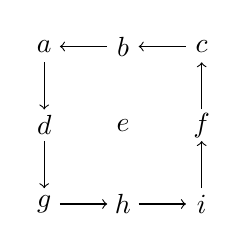
\begin{tikzpicture}
   \draw (0,2) node{$a$};
   \draw (1,2) node{$b$};
   \draw (2,2) node{$c$};
   \draw (0,1) node{$d$};
   \draw (1,1) node{$e$};
   \draw (2,1) node{$f$};
   \draw (0,0) node{$g$};
   \draw (1,0) node{$h$};
   \draw (2,0) node{$i$};
   \draw[->] (0,1.8) -- (0,1.2);
   \draw[->] (0,0.8) -- (0,0.2);
   \draw[->] (0.2,0) -- (0.8,0);
   \draw[->] (1.2,0) -- (1.8,0);
   \draw[->] (2,0.2) -- (2,0.8);
   \draw[->] (2,1.2) -- (2,1.8);
   \draw[->] (1.8,2) -- (1.2,2);
   \draw[->] (0.8,2) -- (0.2,2);   
  \end{tikzpicture}
 \end{center}
 Find a basis for the kernel of $T-1$.  Write down the
 matrix of $T$ with respect to a suitable basis of $M_3\R$,
 and thus calculate the characteristic polynomial of $T$.
\end{exercise}
\begin{solution}
 Consider a matrix $A=\bpm a&b&c \\ d&e&f \\ g&h&i \epm$.
 We have $A\in\ker(T-1)$ iff $A=T(A)$, iff
 \[ \bpm a&b&c \\ d&e&f \\ g&h&i \epm = 
    \bpm b&c&f \\ a&e&i \\ d&g&h \epm
 \]
 This means that $a=b$, $b=c$, $c=f$, $d=a$, $f=i$, $g=d$,
 $h=g$ and $i=h$, which just means that $a=b=c=d=f=g=h=i$
 (but $e$ can be different).  In other words, we have
 \[ A = 
    \bpm a&a&a \\ a&e&a \\ a&a&a \epm = 
    a \bpm 1&1&1 \\ 1&0&1 \\ 1&1&1 \epm + 
    e \bpm 0&0&0 \\ 0&1&0 \\ 0&0&0 \epm
 \]

 {\tiny \[
  E_1 = \bpm 1&0&0\\0&0&0\\0&0&0\epm \hspace{3em}
  E_2 = \bpm 0&0&0\\1&0&0\\0&0&0\epm \hspace{3em}
  E_3 = \bpm 0&0&0\\0&0&0\\1&0&0\epm \hspace{3em}
  E_4 = \bpm 0&0&0\\0&0&0\\0&1&0\epm \hspace{3em}
  E_5 = \bpm 0&0&0\\0&0&0\\0&0&1\epm 
 \] \[
  E_6 = \bpm 0&0&0\\0&0&1\\0&0&0\epm \hspace{3em}
  E_7 = \bpm 0&0&1\\0&0&0\\0&0&0\epm \hspace{3em}
  E_8 = \bpm 0&1&0\\0&0&0\\0&0&0\epm \hspace{3em}
  E_9 = \bpm 0&0&0\\0&1&0\\0&0&0\epm  
 \]}
 These matrices form a basis for $M_3\R$, with the property
 that
 $T(E_1)=E_2$, 
 $T(E_2)=E_3$, 
 $T(E_3)=E_4$, 
 $T(E_4)=E_5$, 
 $T(E_5)=E_6$, 
 $T(E_6)=E_7$, 
 $T(E_7)=E_8$, 
 $T(E_8)=E_1$ and 
 $T(E_9)=E_9$.  The matrix of $T$ with respect to this basis
 is 
 {\tiny \[ U = \bpm 
     0 & 0 & 0 & 0 & 0 & 0 & 0 & 1 & 0 \\
     1 & 0 & 0 & 0 & 0 & 0 & 0 & 0 & 0 \\
     0 & 1 & 0 & 0 & 0 & 0 & 0 & 0 & 0 \\
     0 & 0 & 1 & 0 & 0 & 0 & 0 & 0 & 0 \\
     0 & 0 & 0 & 1 & 0 & 0 & 0 & 0 & 0 \\
     0 & 0 & 0 & 0 & 1 & 0 & 0 & 0 & 0 \\
     0 & 0 & 0 & 0 & 0 & 1 & 0 & 0 & 0 \\
     0 & 0 & 0 & 0 & 0 & 0 & 1 & 0 & 0 \\
     0 & 0 & 0 & 0 & 0 & 0 & 0 & 0 & 1 
    \epm
 \]}
 The characteristic polynomial of $T$ is the determinant of
 $tI-U$, which is $(t^8-1)(t-1)$.
\end{solution}
%------------------------------------------------------------------

\begin{exercise}
 Let $A$ be a $2\tm 2$ matrix over the reals.  Define a map
 $\mu\:M_2\R\xra{}M_2\R$ by $\mu(X)=AX$.  Find the matrix of
 $M$ with respect to a suitable basis of $M_2\R$, and thus
 show that $\det(\mu)=\det(A)^2$.
\end{exercise}
\begin{solution}
 Let $A$ be $\bpm a&b \\ c&d\epm$.  The most convenient
 basis to use is as follows:
 \[ E_1 = \bpm 1&0\\0&0\epm \hspace{3em}
    E_2 = \bpm 0&0\\1&0\epm \hspace{3em}
    E_3 = \bpm 0&1\\0&0\epm \hspace{3em}
    E_4 = \bpm 0&0\\0&1\epm.
 \]
 (It would be more usual to have $E_2$ and $E_3$ the other
 way around, but in this exercise that makes the picture a
 little less clear.)  We then have
 \begin{align*}
  \mu(E_1) = AE_1 &= \bpm a&0\\ c&0 \epm = aE_1+cE_2 \\
  \mu(E_2) = AE_2 &= \bpm b&0\\ d&0 \epm = bE_1+dE_2 \\
  \mu(E_3) = AE_3 &= \bpm 0&a\\ 0&c \epm = aE_3+cE_4 \\
  \mu(E_4) = AE_4 &= \bpm 0&b\\ 0&d \epm = bE_3+cE_4.
 \end{align*}
 This means that the matrix of $\mu$ is 
 \[ B = \bpm a & b & 0 & 0 \\
             c & d & 0 & 0 \\
             0 & 0 & a & b \\
             0 & 0 & c & d \epm.
 \]
 This gives 
 \[ \det(B) = 
     a \det\bpm d&0&0 \\ 0&a&b \\ 0&c&d \epm - 
     b \det\bpm c&0&0 \\ 0&a&b \\ 0&c&d \epm =
     ad\det\bpm a&b \\ c&d\epm - bc\det\bpm a&b\\ c&d\epm =
     (ad-bc)^2 = \det(A)^2.
 \]
\end{solution}

%------------------------------------------------------------------

\begin{exercise}
 Suppose we have vectors $a=(u,v,w)$ and $b=(x,y,z)$ in
 $\R^3$, with $a\neq 0\neq b$ and $\ip{a,b}=0$.  Define
 matrices $A$, $B$ and $C$ by
 \[ 
  A = \bpm u^2 & uv & uw \\ uv & v^2 & vw \\ uw & vw & w^2 \epm
  \hspace{3em}
  B = \bpm x^2 & xy & xz \\ xy & y^2 & yz \\ xz & yz & z^2 \epm
  \hspace{3em}
  C = A+B.
 \]
 Show that $\img(C)=\spn\{a,b\}$, and thus that $\rank(C)=2$.
\end{exercise}
\begin{solution}
 For any vector $p=(r,s,t)$ we have
 \[ Ar =
    \bpm u^2 & uv & uw \\ uv & v^2 & vw \\ uw & vw & w^2 \epm
    \bpm r \\ s \\ t \epm =
    \bpm u^2r+uvs+uwt \\ uvr+v^2s+vwt \\ uwr+vws+w^2t \epm = 
    (ur+vs+wt) \bpm u \\ v \\ w \epm = \ip{a,p} a.
 \]
 Similarly, we have $Bp=\ip{b,p}b$, so 
 \[ Cp = Ap + Bp = \ip{a,p}a + \ip{b,p}b \in\spn\{a,b\}. \]
 It follows that $\img(C)\leq\spn\{a,b\}$.  Now note that
 $a\neq 0$ so $\ip{a,a}>0$ so we can take $p=a/\ip{a,a}$.
 As $\ip{a,b}=0$, the above gives 
 \[ Cp = \ip{a,a/\ip{a,a}} a = a, \]
 which shows that $a\in\img(C)$.  Similarly we see that
 $b\in\img(C)$, so any linear combination of $a$ and $b$
 must also lie in $\img(C)$, or in other words,
 $\img(C)\leq\spn\{a,b\}$.  We have already proved the
 reverse inclusion, so $\img(C)=\spn\{a,b\}$.  To complete
 the exercise we need to show that $a$ and $b$ are linearly
 independent (so they give a basis for $\img(C)$, so
 $\rank(C)=\dim(\img(C))=2$).  Consider a linear relation
 $\al a+\bt b=0$.  Taking the inner product with $a$ gives
 \[ 0=\ip{0,a}=\ip{\al a+\bt b,a} = \al\ip{a,a}+\bt\ip{a,b} 
     = \al\|a\|^2.
 \]
 As $a\neq 0$ we have $\|a\|^2>0$ and so we must have
 $\al=0$.  Similarly we have $\bt=0$, so $a$ and $b$ are
 linearly independent, as required.
\end{solution}
%------------------------------------------------------------------

\begin{exercise}
 For any real number $a$, we consider the matrix
 $A=\bpm a & a^2 & a^4 \\ a^2 & a^2 & a^4 \\ a^4 & a^4 & a^4 \epm$.
 Find the determinant of $A$, and factorise it.  Using this
 as the first step, determine the rank of $A$ for all $a$.
\end{exercise}
\begin{solution}
 First, we have 
 \[ \det(A) =   a   \det\bpm a^2&a^4 \\ a^4&a^4 \epm 
              - a^2 \det\bpm a^2&a^4 \\ a^4&a^4 \epm 
              + a^4 \det\bpm a^2&a^2 \\ a^4&a^4 \epm =
    (a-a^2)(a^6-a^8) = a^7(1-a)^2(1+a).
 \]
 If $a\not\in\{0,1,-1\}$ we see that $\det(A)\neq 0$ and so
 $\rank(A)=3$.  If $a=0$ then $A$ is the zero matrix and
 $\rank(A)=0$.  If $a=1$ then every entry in $A$ is equal to
 one, so the image of $A$ is spanned by the vector
 $(1,1,1)$, so $\rank(A)=1$.  If $a=-1$ then
 $A=\bpm -1&1&1\\1&1&1\\1&1&1\epm$, so the first two columns
 are linearly independent but the third is equal to the
 second, which shows that $\rank(A)=2$.  In conclusion, we
 have
 \[ \rank(A) = \begin{cases}
                0 & \text{ if } a=0 \\
                1 & \text{ if } a=1 \\
                2 & \text{ if } a=-1 \\
                3 & \text{ otherwise }
               \end{cases}
 \]
\end{solution}
%------------------------------------------------------------------
%------------------------------------------------------------------

%------------------------------------------------------------------

\begin{exercise}
 Suppose that $u\in\R^3$ and $\|u\|=1$.  Define
 $\phi\:\R^3\xra{}\R\tm\R^3$ by $\phi(x)=(\ip{u,x},u\tm x)$,
 and define $\psi\:\R\tm\R^3$ by $\psi(t,y)=tu-y$.  Simplify
 $\psi(\phi(x))$, and deduce that $\ker(\phi)=0$.  Find
 $\ker(\psi)$.  
\end{exercise}
\begin{solution}
 
\end{solution}
%------------------------------------------------------------------

\begin{exercise}
 Let $A$ be a matrix of the form
 $\bpm p & 1-p \\ 1-q & q\epm$, with $0<p,q<1$.  Find an
 invertible matrix $P$ and a diagonal matrix $D$ such that
 $P^{-1}AP=D$.  
\end{exercise}
\begin{solution}
 The diagonal entries in $D$ will be the eigenvalues of $A$,
 and the columns of $P$ will be the corresponding
 eigenvectors.  To find these, we note that the
 characteristic polynomial is
 \begin{align*}
  \det\bpm t-p & p-1 \\ q-1 & t-q \epm 
   &= (t-p)(t-q) - (p-1)(q-1) 
    = t^2 - pt - qt + pq - pq + p + q - 1 \\
   &= t^2-(p+q)t+(p+q-1) 
    = (t-1)(t-p-q+1).
 \end{align*}
 The eigenvalues are thus $1$ and $p+q-1$, so
 $D=\bpm p+q-1&0\\0&1\epm$.  It is easy to see that
 $\bsm 1\\1\esm$ is an eigenvector of eigenvalue $1$.  Next,
 put 
 \[ B = (p+q-1)I - A = \bpm q-1 & p-1 \\ q-1 & p-1 \epm. \]
 We see that $B\bsm 1-p\\ q-1\esm=\bsm 0\\ 0\esm$, so
 $\bsm 1-p\\ q-1\esm$ is an eigenvector of $A$ with
 eigenvalue $p+q-1$.  Our matrix $P$ is thus
 $\bpm 1-p&1\\q-1&1\epm$.  As a check, we note that 
 $\det(P)=2-p-q$ (which is nonzero, as $0<p,q<1$) and so 
 \[ P^{-1} = \frac{1}{2-p-q}\bpm 1 & -1 \\ 1-q & 1-p \epm. \]
\end{solution}
%------------------------------------------------------------------

\begin{exercise}
 Define
 \begin{align*}
  V &= \{f\in\R[x]_{\leq 2} \st \int_{-1}^0 f(x)\,dx=0\} \\
  W &= \{f\in\R[x]_{\leq 2} \st \int_0^1    f(x)\,dx=0\}.
 \end{align*}
 Find bases for $V$, $W$ and $V\cap W$.  Show that
 $V+W=\R[x]_{\leq 2}$.
\end{exercise}
\begin{solution}
 We find that 
 \begin{align*}
  V &= \{ax^2+bx+c\st a/3-b/2+c=0\} \\
  W &= \{ax^2+bx+c\st a/3+b/2+c=0\}.
 \end{align*}
 It follows that $\{1-3x^2,1+2x\}$ is a basis for $V$, and
 $\{1-3x^2,1-2x\}$ is a basis for $W$, and $\{1-3x^2\}$ is a
 basis for $V\cap W$.
\end{solution}
%------------------------------------------------------------------

\begin{exercise}
 Put
 \begin{align*}
  V &= \{A\in M_2\R\st A\bpm 1\\1\epm = 0 \} \\
  W &= \{A\in M_2\R\st \bpm 1&1\epm A = 0 \}. 
 \end{align*} 
 Find bases for $V$, $W$ and $V\cap W$.
\end{exercise}
\begin{solution}
 Consider a matrix $A=\bpm a&b \\ c&d\epm$.  We have $A\in V$ iff
 $\bpm a+b\\ c+d\epm=\bpm 0\\0\epm$, or equivalently $b=-a$ and
 $d=-c$.  In that case we have
 \[ A = \bpm a&-a\\ c&-c\epm = 
        a\bpm 1&-1\\0&0\epm + c\bpm 0&0\\1&-1 \epm.
 \]
 Using this, we see that the matrices $P_1=\bpm 1&-1\\0&0\epm$ and
 $P_2=\bpm 0&0\\1&-1\epm$ give a basis for $V$.  Similarly, we have
 $\bpm 1&1\epm A=\bpm a+c&b+d\epm$, which vanishes iff $A$ has
 the form 
 \[ A = \bpm a&b\\ -a&-b\epm =
     a\bpm 1&0\\-1&0\epm + b\bpm 0&1\\ 0&-1\epm.
 \]
 Using this, we see that the matrices $Q_1=\bpm 1&0\\-1&0\epm$ and
 $Q_2=\bpm 0&1\\0&-1\epm$ give a basis for $W$.  Finally, we see
 that $A\in V\cap W$ iff $b=-a$ and $d=-c$ and $c=-a$ and $d=-b$,
 or equivalently $a=d=-b=-c$, which means that
 $A=a\bpm 1&-1\\-1&1\epm$.  It follows that the single matrix
 $\bpm 1&-1\\-1&1\epm=P_1-P_2=Q_1-Q_2$ gives a basis for
 $V\cap W$.
\end{solution}
%------------------------------------------------------------------

\begin{exercise}
 For each $k>0$ we define $r_k\in C[0,1]$ by $r_k(x)=1/(x+k)$. 
 Show that these are linearly independent in $C[0,1]$.
\end{exercise}
\begin{solution}
 \textbf{Find a good proof not using analytic continuation, and 
 include some hints in the question.}
\end{solution}
%------------------------------------------------------------------

\begin{exercise}
 Put 
 \begin{align*}
  V &= \{\text{ symmetric $3\tm 3$ real matrices }\}  \\
    &= \{A\in M_3\R\st A^T=A\} \\
  W &= \{\text{ homogeneous quadratic polynomials in $x,y,z$}\} \\
    &= \{px^2+qxy+rxz+sy^2+tyz+uz^2\st p,\dotsc,u\in\R\}.
 \end{align*}
 Define $\phi\:V\to W$ by 
 \[ \phi(A) = \bpm x & y & z \epm A
              \bpm x \\ y \\ z \epm 
 \]
 Show that this is an isomorphism.
\end{exercise}
\begin{solution}
 Any element $A\in V$ has the form 
 \[ A = \bpm a & b & c \\ b & d & e \\ c & e & f \epm. \]
 For such $A$ we have 
 \[ \phi(A) = 
     \bpm x & y & z \epm 
     \bpm a & b & c \\ b & d & e \\ c & e & f \epm
     \bpm x \\ y \\ z \epm = 
     ax^2+2bxy+2cxz+dy^2+2eyz+fz^2    
 \]
 Now define $\psi\:W\to V$ by 
 \[ \psi(px^2+qxy+rxz+sy^2+tyz+uz^2) =
   \bpm p   & q/2 & r/2 \\
        q/2 & s   & t/2 \\
        r/2 & t/2 & u      \epm.
 \]
 We find that $\psi(\phi(A))=A$ for all $A\in V$, and
 $\phi(\psi(Q))=Q$ for all $Q\in W$, so $\phi$ and $\psi$ are 
 isomorphisms.
\end{solution}
%------------------------------------------------------------------

\begin{exercise}
 Let $V_0$ be the set of functions $f(x)$ of the form
 \[ a_0 + a_1\ln(x) + a_2\ln(x)^2 + \dotsb + a_n\ln(x)^n \]
 for some $n\geq 0$ and some constants $a_0,\dotsc,a_n\in\R$.
 In other words, the functions in $V_0$ have the form $p(\ln(x))$ 
 for some polynomial $p(t)\in\R[t]$.  Next, let $V_m$ be the set 
 of functions of the form $x^mp(\ln(x))$ for some polynomial $p$,
 so for example, the function $f(x)=x^2(1+\ln(x)+9\ln(x)^4)$ is
 a typical element of $V_2$.  Show that differentiation gives a
 homomorphism $D\:V_m\to V_{m-1}$, which is an isomorphism except
 when $m=0$. 
\end{exercise}
\begin{solution}
 
\end{solution}
%------------------------------------------------------------------

\begin{exercise}
 Define a map 
 \[ \phi\:\R[x,y]_{\leq 2} \to \R[x]_{\leq 2} \tm \R[x]_{\leq 2}
 \]
 by 
 \[ \phi(f)(x) = (f(x,x), f(x,-x)).
 \]
 Find bases for the kernel and image of $\phi$.
\end{exercise}
\begin{solution}
 The space $\ker(\phi)$ is one-dimensional, with basis
 $\{x^2-y^2\}$.  The elements
 \[ (1,1), (x,0), (0,x), (x^,0), (0,x^2) \]
 give a basis for $\img(\phi)$.
\end{solution}
%------------------------------------------------------------------

\begin{exercise}
 Define a map $H\:\R[x,y]_{\leq 2}\xra{}M_2\R$ (called the Hessian)
 by 
 \[ H(u) =
   \bpm
    u_{xx}(0,0) & u_{xy}(0,0) \\ u_{xy}(0,0) & u_{yy}(0,0) 
   \epm
 \]
 Find bases for $\ker(H)$ and $\img(H)$.
\end{exercise}
\begin{solution}
 Any element of $u\in\R[x,y]_{\leq 2}$ has the form
 \[ u(x,y)= a + bx + cy + dx^2 + exy + fy^2 \]
 for some $a,b,\dotsc,f\in\R$.  We then have
 \[ H(u) = \bpm 2d & e \\ e & 2f\epm =
     2d\bpm 1&0\\0&0\epm + 
     e\bpm 0&1\\1&0\epm +
     2f\bpm 0&0\\0&1 \epm.
 \]
 It follows that the matrices $\bpm 1&0\\0&0\epm$,
 $\bpm 0&1\\1&0\epm$ and $\bpm 0&0\\0&1\epm$ give a basis for 
 $\img(H)$.  In the above we have $H(u)=0$ iff $d=e=f=0$, or
 equivalently, $u$ actually has degree $\leq 1$.  This means
 that $\{1,x,y\}$ is a basis for $\ker(H)$.
\end{solution}
%------------------------------------------------------------------

%------------------------------------------------------------------


\begin{exercise}
 Give a basis for the space 
 \[ V = \{A\in M_3\R\st A = A^T \text{ and } \trace(A)=0\}.
 \]
\end{exercise}
\begin{solution}
 Any matrix $A\in M_2\R$ lies in $V$ iff it has the form 
 \begin{align*}
  A &= \bsm a & b & c \\ b & d & e \\ c & e & -a-d \esm \\
    &= a \bsm 1&0&0 \\ 0&0&0 \\ 0&0&-1 \esm + 
       b \bsm 0&1&0 \\ 1&0&0 \\ 0&0&0 \esm +
       c \bsm 0&0&1 \\ 0&0&0 \\ 1&0&0 \esm + 
       d \bsm 0&0&0 \\ 0&1&0 \\ 0&0&-1 \esm
 \end{align*}
 for some $a,b,c,d\in\R$.  It follows that the matrices
 \[    \bsm 1&0&0 \\ 0&0&0 \\ 0&0&-1 \esm,
       \bsm 0&1&0 \\ 1&0&0 \\ 0&0&0 \esm,
       \bsm 0&0&1 \\ 0&0&0 \\ 1&0&0 \esm, 
       \bsm 0&0&0 \\ 0&1&0 \\ 0&0&-1 \esm
 \]
 span $V$, and they are clearly linearly independent, so
 they form a basis for $V$.
\end{solution}
%------------------------------------------------------------------

%------------------------------------------------------------------

\begin{exercise}
 Suppose we are given $u,v,q>0$.  Define a bilinear form on
 $\R[x]_{\leq 2}$ by
 \[ \ip{f,g} = u f(-q)g(-q) + v f(0)g(0) + u f(q)g(q). \]
 Show that this is an inner product.  Find $u$, $v$ and $q$
 such that $\ip{f,g}=9\int_{-1}^1 f(t)g(t)\,dt$ for all
 $f,g\in\R[x]_{\leq 2}$.
\end{exercise}
\begin{solution}
 The solution is $u=5$, $v=8$ and
 $q=\sqrt{3/5}=\sqrt{15}/5$.  This can be found using Maple
 with the following steps:
 \begin{verbatim}
  b := (f,g) -> u*f(-q)*g(-q) + v * f(0)*g(0) + u*f(q)*g(q);
  f := (t) -> a0+a1*t+a2*t^2;
  g := (t) -> b0+b1*t+b2*t^2;
  d := expand(b(f,g) - 9*int(f(t)*g(t),t=-1..1));
  _EnvExplicit := true;
  solve({coeffs(d,{a0,a1,a2,b0,b1,b2}),q>0},{u,v,q});
 \end{verbatim}
\end{solution}
%------------------------------------------------------------------

%------------------------------------------------------------------

%------------------------------------------------------------------

%------------------------------------------------------------------

%------------------------------------------------------------------

\begin{exercise}
 Investigate the Haar basis. 
\end{exercise}
\begin{solution}
 
\end{solution}
%------------------------------------------------------------------

\begin{exercise}
 Define a linear map $\phi\:\R[x]_{\leq 2}\xra{}\R^3$ by 
 \[ \phi(f) = \bsm \int_0^1 f(x)\,dx, \;
                   \int_1^2 f(x)\,dx, \;
                   \int_2^3 f(x)\,dx \esm 
 \]
 Show that this is an isomorphism.
\end{exercise}
\begin{solution}
 The effect of $\phi$ on the basis $1,x,x^2$ is as follows:
 \begin{align*}
  \phi(1)   &= \bpm 1 & 1 & 1 \epm \\
  \phi(x)   &= \bpm 1/2 & 3/2 & 5/2 \epm \\
  \phi(x^2) &= \bpm 1/3 & 3 & 19/3 \epm
 \end{align*}
 The matrix of $\phi$ with respect to the obvious bases is
 thus 
 \[ A =
     \bpm 1 & 1/2 & 1/3 \\ 1 & 3/2 & 3 \\ 1 & 5/2 & 19/3 \epm.
 \]
 By hand or by Maple, we can check that $\det(A)=2\neq 0$,
 so $A$ is an invertible matrix, so $\phi$ is an
 isomorphism. 
\end{solution}
%------------------------------------------------------------------

\begin{exercise}\label{ex-check-dependence}
 For each of the following lists of vectors, say (with justification) whether
 they are linearly independent, whether they span $\R^3$,
 and whether they form a basis of $\R^3$.  (If you
 understand the concepts involved, you should be able to do
 this by eye, without any calculation.)
 \begin{itemize}
  \item[(a)] $\vu_1=\bsm 1\\2\\3\esm$, 
             $\vu_2=\bsm 2\\4\\6\esm$,
             $\vu_3=\bsm 3\\6\\9\esm$.
  \item[(b)] $\vv_1=\bsm 1\\0\\0\esm$,
             $\vv_2=\bsm 0\\1\\0\esm$,
             $\vv_3=\bsm 0\\0\\1\esm$,
             $\vv_4=\bsm 1\\1\\1\esm$.
  \item[(c)] $\vw_1=\bsm 1\\0\\1\esm$,
             $\vw_2=\bsm 1\\0\\-1\esm$.
  \item[(d)] $\vx_1=\bsm 1\\1\\1\esm$,
             $\vx_2=\bsm 1\\1\\0\esm$,
             $\vx_3=\bsm 1\\0\\0\esm$.
 \end{itemize}
\end{exercise}
\begin{solution}
 \begin{itemize}
  \item[(a)] These are linearly dependent, because of the
   relation $\vu_2-2\vu_1=0$.  In each of the $\vu_i$'s the
   $y$ coordinate is twice the $x$ coordinate.  This will
   therefore also be true for anything in the span of the
   $\vu_i$'s.  In particular, the vector $\bsm 1\\0\\0\esm$
   does not lie in the span, so the $\vu_i$'s do not span
   all of $\R^3$.  This means that they do not form a basis.
  \item[(b)] Any list of four vectors in $\R^3$ is
   automatically linearly dependent (and so cannot form a
   basis).  More specifically, the relation
   $\vv_1+\vv_2+\vv_3-\vv_4=0$ shows that the $\vv_i$'s are
   dependent.  These vectors span all of $\R^3$, because any
   vector $\va=\bsm x\\ y\\ z\esm\in\R^3$ can be expressed
   as $\va=x\vv_1+y\vv_2+z\vv_3+0\vv_4$.
  \item[(c)] A list of two vectors can only be linearly
   dependent if one is a multiple of the other, which is
   clearly not the case here, so $\vw_1$ and $\vw_2$ are
   linearly independent.  Moreover, a list of two vectors
   can never span all of $\R^3$.  More explicitly, $\vw_1$
   and $\vw_2$ both have $y$-coordinate equal to zero, so
   the same is true of anything in the span of $\vw_1$ and
   $\vw_2$.  In particular, $\bsm 0\\1\\0\esm$ is not in the
   span.  This shows that $\vw_1$ and $\vw_2$ do not form a
   basis of $\R^3$.
  \item[(d)] The vectors $\vx_1$, $\vx_2$ and $\vx_3$ are
   linearly independent and span $\R^3$, so they form a
   basis.  One way to see this is to write down the matrix
   $A=\bsm 1&1&1\\1&1&0\\1&0&0\esm$ whose columns are
   $\vx_1$, $\vx_2$ and $\vx_3$, and observe that it
   row-reduces almost instantly to the identity.
   Alternatively, we must show that for any vector
   $\va=\bsm x\\ y\\ z\esm\in\R^3$, there are unique real
   numbers $\lm,\mu,\nu$ such that 
   \[ \bsm x\\ y\\ z\esm =
       \lm\bsm 1\\1\\1\esm +
       \mu\bsm 1\\1\\0\esm +
       \nu\bsm 1\\0\\0\esm.
   \] 
   This equation is equivalent to $\lm+\mu+\nu=x$ and
   $\lm+\mu=y$ and $\lm=z$.  It is easy to see that there is
   indeed a unique solution, namely $\lm=z$ and $\mu=y-z$ and
   $\nu=x-y$. 
 \end{itemize}
\end{solution}
%------------------------------------------------------------------


\begin{exercise}
 Define a map $\pi\:\R^3\to\R^2$ by 
 \[ \pi\bsm x\\ y\\ z \esm =
     \bsm 2x - y - z \\ \sqrt{3}(y-z) \esm
 \]
 Investigate $\ker(\pi)$, $\img(\pi)$, $\pi^*$, $\pi\pi^*$,
 $\pi^*\pi$.  
\end{exercise}
\begin{solution}
 $\pi$ is surjective, with kernel spanned by $[1,1,1]^T$.  We have
 $\pi\pi^*=6\iota_2$, and $\pi^*\pi=6\iota_3-2\phi_J$, where
 $J_{ij}=1$ for all $i$ and $j$.
\end{solution}

\end{document}
